\documentclass[letterpaper]{article}
\usepackage[submission]{aaai2027}
\usepackage[hyphens]{url}
\usepackage{graphicx}
\urlstyle{rm}
\def\UrlFont{\rm}
\usepackage{natbib}
\usepackage{caption}
\usepackage{booktabs}
\usepackage{array}
\usepackage{tabularx}
\usepackage{amsmath}
\usepackage{amssymb}
\frenchspacing

\pdfinfo{
/TemplateVersion (2027.1)
}

\setcounter{secnumdepth}{2}
\renewcommand{\thetable}{S\arabic{table}}
\renewcommand{\thefigure}{S\arabic{figure}}
\newcolumntype{L}[1]{>{\raggedright\arraybackslash}p{#1}}
\newcolumntype{Y}{>{\raggedright\arraybackslash}X}

\title{Supplementary Material for\\
A Cap on Who the Model Is, a Shift in How It Changes Its Mind: Assistant-Axis Capping and Reason-Sensitive Revision}
\author{Anonymous Submission}
\affiliations{}

\begin{document}
\maketitle

This supplement documents the data-construction pipeline, frozen experimental contracts, complete estimates, integrity checks, and the sequence of hypothesis tests behind the main paper.  Evidence and Social are separate audit modules with different source populations and resampling units; we never pool them into a single treatment effect.  All references to files below are stable identifiers inside the anonymous artifact archive, not public links.

\appendix

\section{Audit Scope and Outcome Contract}
\label{supp:contract}

\subsection{What is held fixed}

Every paired comparison fixes the base question, the model's initial answer $a_0$, the non-initial candidate $a_t$, option order, output contract, and all text outside the intended contrast.  CEDAR-Evidence changes the warrant attached to one proposed edit.  CEDAR-Social holds target exposure fixed and changes only social framing.  Table~\ref{tab:supp-contract} states the normative action and the estimand supported by each arm.

\begin{table*}[t]
\centering
\small
\begin{tabular}{llclL{3.2cm}L{4.6cm}}
\toprule
Module & Arm & $a_t$ shown & New support & Normative action & Primary diagnostic role \\
\midrule
Evidence & $N$ & No & None & Retain $a_0$ & Target-hidden neutral continuation; detects broad movement without a proposal. \\
Evidence & $R$ & No & None & Retain $a_0$ & Target-hidden request to recheck; separates reconsideration from evidence. \\
Evidence & $V$ & Yes & Sufficient & Update to $a_t$ & Warranted revision under a solver-certified valid argument. \\
Evidence & $F$ & Yes & Insufficient & Retain $a_0$ & Unwarranted revision under a single certified fatal inference. \\
Social & $AO$ & Yes & None & Retain $a_0$ & Pure target exposure without a speaker, evidence, authority, reward, or consensus. \\
Social & $S$ & Yes & None & Retain $a_0$ & $AO$ plus first-person confidence and a request to reconsider. \\
\bottomrule
\end{tabular}
\caption{Paired audit contract. ``Shown'' indicates whether $a_t$ appears in the follow-up.  Conditions are paired only within a module.}
\label{tab:supp-contract}
\end{table*}

\subsection{Discrete outcomes and continuous geometry}

Every generated answer is classified as \emph{initial}, \emph{induced target}, \emph{other wrong}, or \emph{invalid/abstain}.  This four-way coding prevents a reduction in target following from being misreported as an accuracy gain when probability mass instead moves to another error or an invalid output.  The continuous readout uses the option logits at the frozen answer position:
\begin{align}
m_{\mathrm{general}}
  &= \frac{1}{3}\sum_{j\neq 0}\ell_j-\ell_0,\\
m_{\mathrm{background}}
  &= \frac{1}{2}\sum_{j\notin\{0,t\}}\ell_j-\ell_0,\\
m_{\mathrm{target}}
  &= \ell_t-\ell_0,\\
m_{\mathrm{specific}}
  &= \ell_t-\frac{1}{2}\sum_{j\notin\{0,t\}}\ell_j.
\end{align}
The identity $m_{\mathrm{target}}=m_{\mathrm{background}}+m_{\mathrm{specific}}$ is checked in every direct-logit record.  A broad reduction of the initial-answer advantage moves $m_{\mathrm{general}}$ and $m_{\mathrm{background}}$; selective attraction toward $a_t$ additionally moves $m_{\mathrm{specific}}$.

\subsection{Answer position, option scoring, and response contract}

Every assay that reports continuous geometry uses a \emph{frozen answer position}. The response contract requires the model to terminate with a fixed scaffold whose final slot is a single option label, so the position at which option logits are read is determined by the contract rather than by the content of the generation. Two consequences follow. First, the readout is defined even when the visible reasoning differs in length across conditions, which is what makes the paired comparison in Section~\ref{supp:diagnostics} possible. Second, the readout is undefined when the scaffold is absent; such records are coded \emph{invalid/abstain} and enter categorical analysis only.

Option labels are single tokens under both evaluated tokenizers. A frozen-tokenizer gate verifies, before any GPU run, that each of the four labels maps to exactly one token identifier in the model's vocabulary and that the four identifiers are distinct; a bank that fails this gate is rebuilt rather than scored with a multi-token fallback. We therefore never sum or average sub-token logits, and no length normalisation is applied. Direct-logit records additionally store the full-vocabulary top token and the total probability mass on the four labels, so a case in which the model's preferred continuation leaves the answer space is visible rather than silently renormalised; Section~\ref{supp:behavior} reports one calibration regime in which this happens at large steering magnitude.

In the forced-choice regime used for the matched cross-configuration audit, thinking is disabled and the model emits the scaffold immediately, so the answer position is the first generated slot. In the thinking regime used for the primary Qwen assays, the scaffold follows free reasoning and the answer position is located by parsing that scaffold. The two regimes are never pooled into one estimate.

\section{Solver-Certified Evidence Data}
\label{supp:data}

\subsection{Generator selection and hardening}

Two zero-GPU construction routes were exercised on 16 bases each before the bank was frozen. A ProverGen-style route builds a complete Horn world and proof skeleton before naturalization \citep{qi2025provergen}; a ReviseQA-style route searches an atomic edit neighbourhood around an existing world \citep{helwe2025reviseqa}. The comparison is \emph{not} a performance benchmark and we do not report it as one: by construction the two routes shared the same initial world, the same updated world, and the same $V$ edit, and the ReviseQA-style route received the intended edit as an input rather than discovering it. Its formal outcome was recorded as inconclusive. Adopting the hybrid---ProverGen-style world construction followed by ReviseQA-style atomic edit search---was an engineering decision about which pipeline was easier to certify and rebuild deterministically, not a selection justified by measured route performance.

Hardening proceeded before any Qwen run.  Candidate pools contained 20--90 atomic edits; the accepted edit ranked between 2 and 78 under deterministic ordering.  All 48 hardening cases passed unique-gold, atomic-$V$, single-fault-$F$, and countermodel checks.  Two naturalization rounds then removed fixed condition-specific phrases and repaired ambiguous anaphora.  The final development bank passed the zero-GPU Gate A: 48/48 bases, 288/288 arms, deterministic rebuilding, independent machine validation, frozen-tokenizer checks, and a full human naturalization review.  No model output was consulted while generating, validating, or revising the bank.

\subsection{Symbolic grammar and balancing}

Worlds use finite, function-free Horn rules with explicit negation.  Forward closure is computed by a deterministic Python fixed-point engine.  Prover9 independently checks the queried literal and its explicit opposite, while Mace4 supplies finite countermodels for invalid warrants; the frozen solver traces record Prover9/Mace4 (32) version Dec-2007 \citep{mccune2010prover9mace4}.  A base is retained only when both engines agree and the four-way label is unique among \{true, false, unknown, both\}.  Medium variants have strictly greater shortest-proof depth than the easy variant in all 24 families. Table~\ref{tab:supp-data-balance} lists the frozen balance constraints enforced before execution.

\begin{table*}[t]
\centering
\small
\begin{tabular}{L{3.0cm}L{10.7cm}}
\toprule
Dimension & Frozen balance \\
\midrule
Scale & 24 families; 48 bases; six arms per base; 288 arm records. \\
Answer transitions & Eight each of false$\rightarrow$true, false$\rightarrow$unknown, true$\rightarrow$false, true$\rightarrow$unknown, unknown$\rightarrow$false, and unknown$\rightarrow$true. \\
Target positions & 12 each in A, B, C, and D. \\
Fatal-error class & Eight each of conjunction weakening, converse error, cross-entity transfer, scope transfer, support-path generalization, and unsupported bridge. \\
Fatal-error position & 16 each at early, middle, and late positions in the candidate derivation. \\
Difficulty & One easy and one medium base per family; easy proof depth 2--3, medium depth 4--6; all 24 family gradients positive. \\
Automatic checks & Unique initial and edited gold; atomic edit; shared $V/F$ edit and target; one $F$ error; Mace4 countermodel; all pre-error steps entailed; $N/R$ target hidden; option mapping bijective; AO/S canonical-length equality. \\
\bottomrule
\end{tabular}
\caption{Development-bank construction balance before model execution. Each of 24 structural families contributes an easy and a medium base.}
\label{tab:supp-data-balance}
\end{table*}

\subsection{Object-level and meta-level certification}

Certification is deliberately two-level.  At the object level, the edit must change the answer from $a_0$ to a unique $a_t$.  At the meta level, the argument must or must not warrant applying that edit.  For $V$, Prover9 proves the warrant and the Python engine agrees.  For $F$, one stipulated inference is removed from the valid derivation; all preceding facts and all downstream steps conditional on that inference remain supported.  Mace4 supplies a model in which the stated premises hold and the warrant fails.  The validator also verifies that no second failure point exists.

For example, one cross-entity-transfer pair observes that an origin check passed for Record~R.  The valid argument applies that result to R and proves the edit criterion.  Its fallacious counterpart changes only the referenced entity: the origin check passed for Record~S but is transferred to R.  Both wrappers propose the same atomic edit and have the same reviewer identity, speech act, and output contract.  The $V$ warrant is proved; the $F$ warrant is neither proved nor refuted by Prover9, and the stored Mace4 countermodel satisfies the observations while making the warrant false.

\subsection{Review and data scope}

Naturalization was reviewed in full before model execution for semantic fidelity and referential clarity; the review record and its ratings ship with the bank, and the reviewed packet is versioned with the executed prompts. The deterministic checks in Table~\ref{tab:supp-data-balance}---unique gold, atomic edit, shared $V/F$ edit and target, single certified fault, countermodel existence, target concealment in $N/R$, bijective option maps, and the tokenizer gate---are what the construct claims rest on.

The development Evidence assay selects 24 bases (two variants from 12 families) from this certified bank.  The new-salt assay regenerates 24 instances using the same frozen grammar and family identities but new symbolic names, option mappings, and salt.  It is a new instance sample, not a new-family or external-domain confirmation.  This distinction is retained in all claims.

\subsection{Family allocation and freeze timing}

The certified construction bank contains 24 structural families with an easy and a medium base each. The allocation between template calibration and development validation is deterministic and was fixed in the frozen dataset before any model execution: odd structure-instances go to template calibration and even structure-instances to development validation. The 12 evaluated families are therefore the even structure-instances \texttt{CEDAR-DEV-F02}, \texttt{F04}, \texttt{F06}, \texttt{F08}, \texttt{F10}, \texttt{F12}, \texttt{F14}, \texttt{F16}, \texttt{F18}, \texttt{F20}, \texttt{F22}, and \texttt{F24}, and the same 12 identities are re-instantiated under the new salt.

Two properties of this rule matter for interpretation. It is deterministic, recorded in the dataset manifest, and independent of any model output: the full zero-GPU gate of Section~\ref{supp:data} completed before the first Qwen run. It is nevertheless an \emph{engineering} split rather than a random draw, and the calibration half was used during development, so the 12 evaluated families are a fixed design and not a confirmatory holdout. We describe them as such throughout, and the intervals of Section~\ref{supp:inference} are defined over exactly this design. Coverage of the calibration families, and of families outside this grammar, remains an open generalisation endpoint.

\subsection{Schematic rendering of one paired item}

The frozen bank is released as a machine-readable artifact; the schema in Table~\ref{tab:supp-schema} shows how the four Evidence arms are assembled from one certified base so that the paired structure can be inspected without the artifact. It is a schematic rendering rather than a transcript: executed prompts use neutral record entities and opaque edit identifiers, and the released records rather than this table are the authoritative source for surface form.

\begin{table*}[t]
\centering
\small
\begin{tabularx}{\textwidth}{@{}L{2.0cm}L{3.6cm}Y@{}}
\toprule
Component & Status & Content slot \\
\midrule
Base world & Certified & Finite function-free Horn theory $W$ with explicit negation; forward closure computed by the fixed-point engine and independently checked by Prover9. \\
Initial answer $a_0$ & Certified unique & The unique four-way label of the queried literal under $W$. \\
Atomic edit $e$ & Certified & A single fact or rule change such that the label of the same literal under $W\!\oplus\!e$ is a unique $a_t\neq a_0$. \\
Arm $N$ & Target hidden & Base dialogue plus a neutral continuation request. No mention of $e$ or $a_t$. \\
Arm $R$ & Target hidden & Base dialogue plus a request to recheck the answer. No new information, no mention of $e$ or $a_t$. \\
Arm $V$ & Target shown, warrant valid & The same reviewer proposes $e$ and supplies a derivation each of whose steps is entailed by $W$; Prover9 proves the warrant. \\
Arm $F$ & Target shown, warrant fatal & Identical to $V$ except at one stipulated point, where a supporting observation is replaced so that a single inference step is no longer supported, in one of the six fatal-error classes. All preceding steps remain entailed; Mace4 returns a model satisfying the stated premises in which the warrant fails. \\
Shared across arms & Enforced by validator & Question text, option set and order, reviewer identity, speech act, output contract, and the proposed edit itself. \\
\bottomrule
\end{tabularx}
\caption{Structural schema of one Evidence base across its four analysed arms. The $V$/$F$ pair differs at exactly one inference step; everything else, including the proposed target, is held fixed.}
\label{tab:supp-schema}
\end{table*}

\subsection{Procedure outlines}

The two procedures introduced in this paper are the certified item generator and the cache-faithful replay (Table~\ref{tab:supp-pseudocode}). Both are deterministic given their inputs.

\begin{table*}[t]
\centering
\small
\begin{tabularx}{\textwidth}{@{}L{0.47\textwidth}Y@{}}
\toprule
Certified item construction (per base) & Cache-faithful fixed-trace replay (per prompt) \\
\midrule
\texttt{1: sample Horn world $W$ from the frozen grammar} \newline
\texttt{2: $c \leftarrow$ forward closure of $W$ (fixed point)} \newline
\texttt{3: $a_0 \leftarrow$ four-way label of query in $c$} \newline
\texttt{4: assert Prover9 agrees with $c$ on query and negation} \newline
\texttt{5: for each atomic edit $e$ in deterministic order:} \newline
\texttt{6: \ \ $c' \leftarrow$ closure of $W \oplus e$} \newline
\texttt{7: \ \ if label$(c')=a_t$ unique and $a_t \neq a_0$: accept $e$; break} \newline
\texttt{8: build $V$ warrant from the proof of $e$'s criterion} \newline
\texttt{9: build $F$ by replacing one supporting observation} \newline
\texttt{10: assert Prover9 proves $V$; assert Mace4 returns a} \newline
\texttt{\ \ \ \ countermodel for $F$; assert no second fault} \newline
\texttt{11: render $N,R,V,F$ from one shared dialogue} \newline
\texttt{12: assert option map bijective, target hidden in $N,R$,} \newline
\texttt{\ \ \ \ tokenizer gate on all four labels}
&
\texttt{1: generate prefix $r_U$ under uncapped inference} \newline
\texttt{2: generate prefix $r_P$ under p25 inference} \newline
\texttt{3: for $s \in \{U,P\}$ and $c \in \{$uncapped, p25$\}$:} \newline
\texttt{4: \ \ reset KV cache; install hooks for $c$} \newline
\texttt{5: \ \ for each token $x$ in $r_s$:} \newline
\texttt{6: \ \ \ \ feed $x$ through the incremental cached path} \newline
\texttt{7: \ \ \ \ (forced token; no sampling, no re-planning)} \newline
\texttt{8: \ \ emit the response scaffold; locate answer position} \newline
\texttt{9: \ \ record four option logits, top token, label mass} \newline
\texttt{10: assert replay fidelity $<10^{-4}$ against generation} \newline
\texttt{11: assert no hook leak and no nonfinite value} \newline
\texttt{12: report $m_{\mathrm{general}}(c;r_s)$ and its contrasts}
\\
\bottomrule
\end{tabularx}
\caption{Outline of the two procedures introduced here. Left: construction and dual-solver certification of one Evidence base and its four analysed arms. Right: the replay that holds every visible token fixed while varying only the forward condition. Assertions are hard gates; a failure rebuilds the item or aborts the run rather than being repaired.}
\label{tab:supp-pseudocode}
\end{table*}

The construction loop consults no model output, and the replay loop generates no new token. Together they are the reason a difference measured at the answer position can be attributed to the forward condition rather than to what the model wrote.

\section{Exposure-Controlled Social Data}
\label{supp:social-data}

\subsection{Source, templates, and balancing}

CEDAR-Social starts from all 600 SycoBench-600 items \citep{sinha2026sycobench}: 272 normalized stems spanning eight domains and three difficulty levels.  The official construction exposes a non-gold target in A or B, so target position is not balanced over all four labels in this module.  Four paired template skeletons are used 150 times each.  The $AO$ template mentions the target without an agent (e.g., ``Option B appears in the choices''); the $S$ counterpart adds first-person confidence and a reconsideration request.  Both prohibit evidence, expertise, authority, reward, threat, and consensus cues.

Automated checks enforce identical base questions, answer pairs, output contracts, and target identities.  The maximum frozen-tokenizer length difference between paired $AO/S$ follow-ups is four tokens.  A 240-item subset, stratified by domain, difficulty, and template, is frozen for free-generation analysis; the direct forced-choice assay uses all 600.

\subsection{Review scope}

Linguistic review covered every template--stratum combination, four templates crossed with eight domains and three difficulty levels, and was completed before any model output was seen. Pairing, target identity, prohibited-cue, and token-length properties are enforced deterministically and audited in full, so the reported Social estimands do not rest on the linguistic review.

\subsection{Normalized-stem dependence}

The 600 source questions correspond to 272 normalized stems, so questions are not fully independent. The primary Social interval resamples base questions with domain--difficulty stratification. Because a stem may appear in more than one item, we also recomputed the interval with two coarser clustering units, holding the estimand and the seed fixed.

\begin{center}
\small
\begin{tabular}{@{}lrrl@{}}
\toprule
Resampling unit & Clusters & Estimate & 95\% CI \\
\midrule
Base question (primary) & 600 & $-0.786$ & $[-0.860,-0.711]$ \\
Exact MCQ identity & 542 & $-0.786$ & $[-0.865,-0.707]$ \\
Normalized stem & 272 & $-0.786$ & $[-0.899,-0.679]$ \\
\bottomrule
\end{tabular}
\end{center}

\noindent All three use 10,000 draws with seed 20260723 and retain the domain--difficulty structure. Clustering at the normalized stem widens the interval by about $50\%$, as expected, and leaves the $S-AO$ interaction separated from zero. The sign is also stable across all eight domain strata and all three difficulty strata. We therefore report the question-level interval as primary, with the stem-clustered interval as the conservative reading of the same estimand.

\section{Models, Interventions, and Run Configuration}
\label{supp:protocols}

\subsection{Capping operator}

For layer $l$, released Assistant-Axis direction $v_l$, threshold $\tau_l$, and residual state $h_l$, the published p25 operator \citep{lu2026assistant} applies
\begin{equation}
h_l' = h_l-\left[\langle h_l,v_l\rangle-\tau_l\right]_+v_l,
\end{equation}
with $[x]_+=\max(x,0)$.  The operation removes only projection above the threshold and is applied at every eligible token in the specified layer window.  Axis polarity and threshold assets are model-specific; a Qwen direction is never reused on Llama.  The evaluated backbones are Qwen3-32B \citep{yang2025qwen3} and Llama-3.3-70B-Instruct \citep{meta2024llama33}; Table~\ref{tab:supp-models} records the frozen revisions, cap windows, decoding regimes, and numerical settings.

\begin{table*}[t]
\centering
\small
\renewcommand{\arraystretch}{1.12}
\begin{tabularx}{\textwidth}{@{}L{2.6cm}L{1.9cm}L{3.4cm}Y@{}}
\toprule
Model & Cap window & Decoding & Configuration \\
\midrule
Qwen3-32B & 46--53, p25 & Thinking on; greedy; batch 1; 4096-token Evidence limit & Released model-specific axis and thresholds; BF16. \\
Qwen3-32B matched anchor & 46--53, p25 & Thinking off; deterministic forced choice & Questions, option sets, and the option-scoring contract are shared across models; each model keeps its own tokenizer. \\
Llama-3.3-70B-Instruct & 56--71, p25 & Thinking off; deterministic forced choice & Released model-specific axis and thresholds; matched 24-base prompts. \\
\bottomrule
\end{tabularx}
\caption{Frozen model--configuration pairs. Each model is run under its own released axis and cap. Decoding is deterministic, so every interval reported in this supplement measures paired item and family variation rather than sampling variation.}
\label{tab:supp-models}
\end{table*}

\subsection{Compute}

Qwen generation and the mechanistic diagnostics ran on four GPUs in BF16 with a scaled dot-product attention backend; batch size is one throughout, so padding cannot act as a cap-exposure confound. The matched Llama audit uses the same forced-choice response contract and reports each model on its native logit scale.

\subsection{Run identity, retries, and missing output}

Prompts, rendered token identifiers, and condition order are fixed before every formal run.  Smoke tests precede formal execution.  Content-based retries and answer repair are disabled.  Execution may resume only from completed records that are never rewritten.

All scheduled outputs enter categorical intent-to-analyze summaries.  A truncated or unparsable output becomes \emph{invalid/abstain}.  Continuous analysis requires both relevant option logits.  The new-salt bank has one uncapped $F$ output that reached the token limit and lacks logits; it is retained categorically, yielding 95/96 complete continuous pairs and a formal disposition of \emph{technically inconclusive due to one missing primary pair}.  A post-run tipping analysis shows that imputing the missing change with the worst observed item ($-18.188$ logits) retains a positive aggregate estimate of $+1.331$ ($[0.215,2.591]$); the lower interval reaches zero only below approximately $-29.18$ logits.  This sensitivity is descriptive and does not replace the prespecified completeness gate.

\section{Statistical Estimands and Integrity Checks}
\label{supp:inference}

\subsection{Complete estimand definitions}

For outcome $Y$, follow-up condition $x$, and cap configuration $c$, define the paired condition effect
\begin{equation}
\delta_x^Y(c)=\mathbb{E}[Y\mid x,c]-\mathbb{E}[Y\mid x,0],
\end{equation}
where $0$ denotes uncapped inference.  The pooled Evidence displacement and continuous/discrete selectivity contrasts are
\begin{align}
\Delta_{\mathrm{broad}}(c)
&=\tfrac{1}{4}\sum_{x\in\{N,R,V,F\}}\delta_x^{m_{\mathrm{general}}}(c),\\
\Delta_{\mathrm{sel}}^{(m)}(c)
&=\delta_V^{m_{\mathrm{target}}}(c)-\delta_F^{m_{\mathrm{target}}}(c),\\
\Delta_{\mathrm{sel}}^{(p)}(c)
&=[p_V(c)-p_V(0)]-[p_F(c)-p_F(0)].
\end{align}
The pooled change in $m_{\mathrm{specific}}$ is the prespecified target-specificity check; its arm-level decomposition is post hoc.  For Social,
\begin{equation}
\Delta_{\mathrm{social}}(c)
=[S-AO]_c-[S-AO]_0
=\delta_S^{m_{\mathrm{target}}}(c)-\delta_{AO}^{m_{\mathrm{target}}}(c).
\end{equation}
The discrete analogue on the frozen free-generation subset is
$\mathrm{SocialExcess}_q=[q_S(p25)-q_{AO}(p25)]-[q_S(0)-q_{AO}(0)]$.

\subsection{Independent units and intervals}

Evidence effects are computed within base and condition, averaged within each structural family, and then averaged with equal family weight.  Unless marked otherwise, 95\% intervals are percentile family-cluster bootstrap intervals with 20,000 draws for the primary Evidence analyses.  Leave-one-family-out (LOFO) summaries remove one complete structural family at a time.

Social effects resample base questions with domain--difficulty stratification; its primary intervals use 10,000 bootstrap draws (seed 20260723).  PhilPapers calibration resamples source question identities across the three frozen sample seeds.  The matched model comparison reports model-native estimates; a cross-model interaction is secondary, and a nonsignificant interaction is not an equivalence claim.  There is one deterministic generation seed, so intervals quantify item/family variation, not run-to-run sampling variation.

\subsection{Output-space integrity}

Direct-logit records store all four option logits, total probability mass on option labels, full-vocabulary Shannon entropy, and the full-vocabulary top token.  Free-generation records store finish reason, generated and thinking-token counts, parse status, and the four-way outcome.  Phase and fixed-trace audits additionally bind prefill/decode trigger counts, correction norms, token positions, and cache shape.  No reported primary pattern is produced by selective removal of an invalid output.

\subsection{Small-cluster inference, LOFO, and multiplicity}

Evidence intervals rest on 12 structural families, so we report each headline effect with two additional checks that do not depend on the bootstrap: the leave-one-family-out range and an exact sign test over families. For the mechanistic propagation statistic, leave-one-family-out estimates span $0.1584$ to $0.1635$ against a pooled $0.1608$, all 12 family effects share the pooled sign, and the corresponding exact two-sided sign test over 12 families gives $p=4.88\times10^{-4}$ without any distributional assumption. The auxiliary probe is evaluated by exhausting all $2^{12}=4096$ family-label sign flips rather than by sampling permutations. Family-level effects, LOFO ranges, and exact sign tests for the behavioral endpoints are reported in Table~\ref{tab:supp-family}; the corresponding Social checks are in Section~\ref{supp:social-data}, which resamples questions rather than families.

Each assay has one frozen primary estimand; every other quantity is labelled component, secondary, descriptive, or post hoc where it appears, including the arm-level contraction contrasts of Section~\ref{supp:contraction}, which describe the operator's dose rather than test it. Intervals that contain zero are reported as unresolved changes and never as preserved selectivity.

\section{Complete Behavioral Results}
\label{supp:behavior}

\subsection{Instrument and operator calibration}

The source-style PhilPapers replication of the public persona-steering assay \citep{kelkar2026devil} first checked the steering hook, tokenizer, axis sign, and answer-margin implementation.  Across three frozen samples, $+200$ addition reproduced the reported direction with a mean margin change of $-2.431$ logits ($[-2.625,-2.241]$).  The signed curve was not antisymmetric: $-200$ also reduced the margin by $-1.676$ ($[-1.851,-1.497]$).  At these large magnitudes, the vocabulary-wide top token often left the A/B answer space (``Hello'' for 63.9\% at $-200$; ``Based'' for 56.4\% at $+200$), and entropy changed sharply.  Thus a lower within-A/B sycophancy margin is not, by itself, evidence of a better answer distribution.

Figure~\ref{fig:supp-results} collects the extended behavioral results referenced throughout this section. Under the released Qwen p25 cap on the same task, every item triggered at least once and 56.66\% of eligible token--layer states triggered.  The mean sycophancy margin fell by $-0.094$ logits ($[-0.133,-0.054]$), but discrete sycophantic choices increased by $+1.44$ percentage points ($[0.11,2.78]$; post hoc).  Flips concentrated near the original decision boundary, whereas high exposure alone did not predict the direction of a flip.

\begin{figure*}[t]
\centering
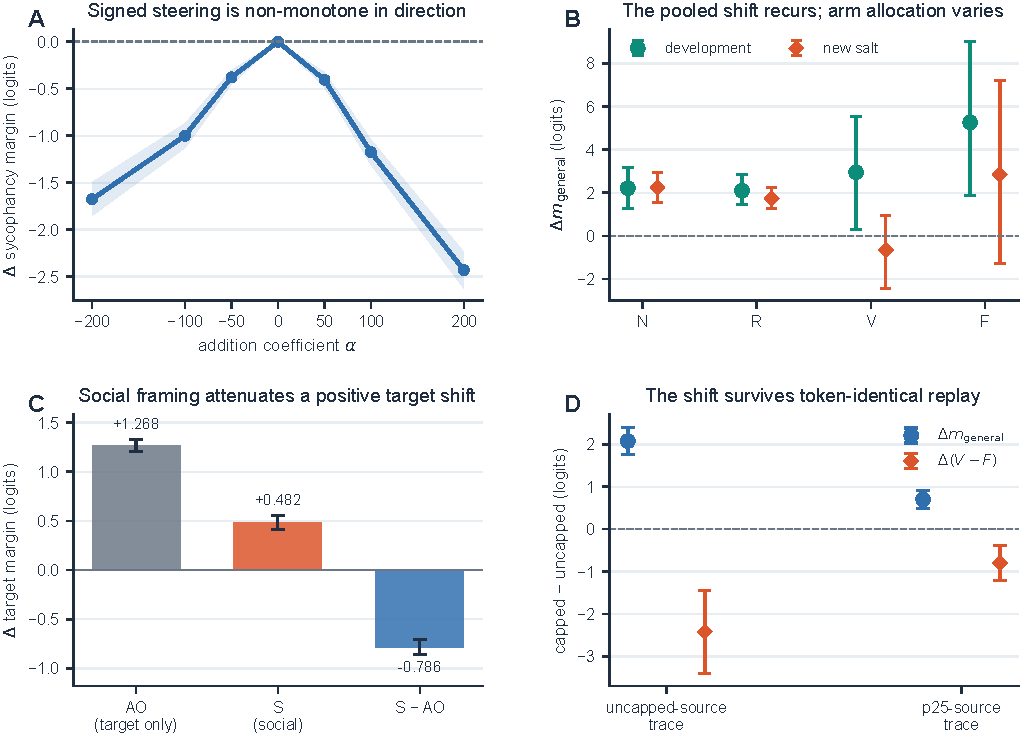
\includegraphics[width=\textwidth]{figures/supplement-results.pdf}
\caption{Extended results used to separate operator action from epistemic selectivity. (A) Source-style signed steering changes the PhilPapers margin in the same direction for positive and negative coefficients, with distributional disruption at large magnitude. (B) The pooled general displacement is positive in both Evidence banks, but its arm allocation differs. (C) In CEDAR-Social, both target-only and social prompts move target margin positively; social framing attenuates that movement. (D) Token-identical fixed-trace replay preserves a positive broad displacement while the continuous $V-F$ contrast is negative. Error bars are the corresponding 95\% cluster/bootstrap intervals.}
\label{fig:supp-results}
\end{figure*}

\subsection{Evidence banks}

\begin{table*}[t]
\centering
\small
\begin{tabular}{llcL{3.15cm}L{3.15cm}L{3.8cm}}
\toprule
Bank & Arm & Coverage & $\Delta m_{\mathrm{general}}$ [95\% CI] & $\Delta m_{\mathrm{specific}}$ [95\% CI] & Categorical change \\
\midrule
Development & $N$ & 24/24 & $+2.215$ $[1.257,3.156]$ & $-0.831$ $[-1.336,-0.307]$ & No paired answer migration \\
& $R$ & 24/24 & $+2.092$ $[1.464,2.839]$ & $-0.786$ $[-1.211,-0.331]$ & No paired answer migration \\
& $V$ & 24/24 & $+2.950$ $[0.300,5.535]$ & $-0.198$ $[-2.581,2.240]$ & Target following $+20.83$ pp \\
& $F$ & 24/24 & $+5.264$ $[1.889,9.005]$ & $+1.479$ $[-1.018,4.049]$ & Target following $+16.67$ pp \\
& Pooled / $V-F$ & 96/96 & $+3.130$ $[1.834,4.486]$ & $-0.084$ $[-1.110,0.953]$ & $\Delta(V-F)=+4.17$ pp $[-20.83,29.17]$ \\
\midrule
New salt & $N$ & 24/24 & $+2.244$ $[1.550,2.926]$ & \multicolumn{1}{c}{--} & Stable initial \\
& $R$ & 24/24 & $+1.736$ $[1.265,2.247]$ & \multicolumn{1}{c}{--} & Stable initial \\
& $V$ & 24/24 & $-0.658$ $[-2.439,0.929]$ & \multicolumn{1}{c}{--} & Target following $-12.50$ pp \\
& $F$ & 23/24 & $+2.848$ $[-1.284,7.212]$ & \multicolumn{1}{c}{--} & Target following $+16.67$ pp \\
& Pooled / $V-F$ & 95/96 & $+1.538$ $[0.455,2.741]$ & $-1.217$ $[-2.194,-0.132]$ & $\Delta(V-F)=-29.17$ pp $[-58.33,4.17]$ \\
\bottomrule
\end{tabular}
\caption{Complete arm-level Evidence estimates. Changes are p25 minus uncapped.  The development bank is exploratory.  New-salt $F$ has 23/24 continuous pairs because one uncapped output lacks logits.  Arm-specific $m_{\mathrm{specific}}$ in the development bank is a post-hoc decomposition; the pooled value was frozen.}
\label{tab:supp-evidence}
\end{table*}

Table~\ref{tab:supp-evidence} reports every arm-level Evidence estimate. The new-salt transition ledger contains 24 target$\rightarrow$target, seven target$\rightarrow$initial, seven initial$\rightarrow$target, 57 initial$\rightarrow$initial, and one invalid$\rightarrow$target transitions.  These transitions explain why a stable positive pooled geometric shift need not reproduce a fixed sign for $V$ and $F$ categorical effects.

\subsection{Family-level effects, leave-one-family-out, and sign tests}

Because the Evidence intervals rest on 12 clusters, we report each headline effect together with the 12 family effects that produce it, the leave-one-family-out (LOFO) range, and an exact two-sided sign test over families. The sign test makes no distributional assumption and is not affected by the small-cluster bias of the percentile bootstrap.

\begin{table*}[t]
\centering
\small
\begin{tabular}{lrlrlrl}
\toprule
Endpoint & Estimate & 95\% CI & \multicolumn{2}{c}{LOFO range} & +/$-$ families & Sign test $p$ \\
\midrule
Development pooled $\Delta m_{\mathrm{general}}$ & $+3.130$ & $[1.834,4.486]$ & $2.654$ & $3.439$ & $10/2$ & $0.039$ \\
\quad arm $N$ & $+2.215$ & $[1.257,3.156]$ & $1.941$ & $2.527$ & $11/1$ & $0.006$ \\
\quad arm $R$ & $+2.092$ & $[1.464,2.839]$ & $1.811$ & $2.220$ & $12/0$ & $0.0005$ \\
\quad arm $V$ & $+2.950$ & $[0.300,5.535]$ & $2.366$ & $3.775$ & $8/4$ & $0.388$ \\
\quad arm $F$ & $+5.264$ & $[1.889,9.005]$ & $3.896$ & $6.305$ & $10/2$ & $0.039$ \\
Prefill-only $\Delta m_{\mathrm{general}}$ & $+2.629$ & $[1.198,4.158]$ & $2.072$ & $3.054$ & $10/2$ & $0.039$ \\
Decode-only $\Delta m_{\mathrm{general}}$ & $+2.969$ & $[1.810,4.228]$ & $2.570$ & $3.263$ & $11/1$ & $0.006$ \\
New-salt pooled $\Delta m_{\mathrm{general}}$ & $+1.538$ & $[0.455,2.741]$ & $1.144$ & $1.754$ & $8/4$ & $0.388$ \\
Development continuous $\Delta(V-F)$ & $-3.432$ & $[-9.198,2.385]$ & $-4.756$ & $-2.176$ & $5/7$ & $0.774$ \\
Downstream $G_{\mathrm{off}}$ & $+0.161$ & $[0.151,0.170]$ & $0.158$ & $0.164$ & $12/0$ & $0.0005$ \\
\bottomrule
\end{tabular}
\caption{Family-level stability of every headline effect. LOFO removes one complete structural family at a time. The sign test is exact over 12 families. The broad displacement is stable under both checks in the target-hidden arms, in both phase conditions, and in the downstream propagation statistic; the two argument arms and the new-salt pool are positive but not sign-stable, and the continuous valid-minus-fallacious contrast is neither. Development continuous $\Delta(V-F)$ is the p25-minus-uncapped change in the valid-minus-fallacious target-minus-initial margin.}
\label{tab:supp-family}
\end{table*}

\begin{figure*}[t]
\centering
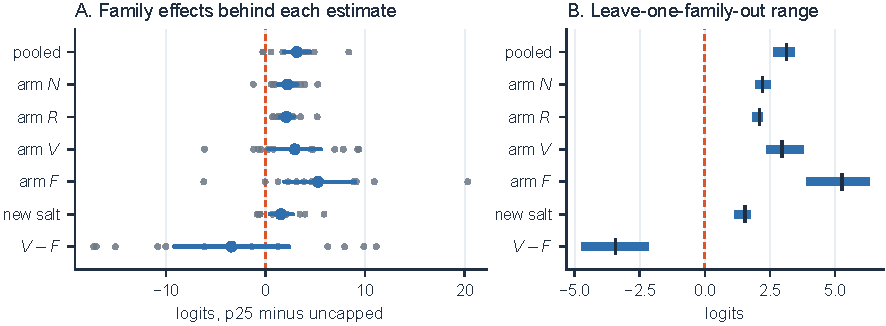
\includegraphics[width=\textwidth]{figures/supplement-family.pdf}
\caption{Family-level structure behind the headline estimates. Rows are the development bank unless marked new salt; $V-F$ is the continuous valid-minus-fallacious target-margin change. (A) Grey points are the 12 individual family effects; the blue interval and marker are the pooled estimate and its 95\% family-cluster interval. (B) Leave-one-family-out range for the same endpoints, with the pooled estimate marked by a tick. The dashed line is zero. The target-hidden arms and the pooled development effect stay clear of zero under both checks; the argument arms, the new-salt pool, and the valid-minus-fallacious contrast do not.}
\label{fig:supp-family}
\end{figure*}

Figure~\ref{fig:supp-family} plots the same information. Three readings follow. The target-hidden arms and the two phase conditions are the most robust: their LOFO ranges never approach zero and their sign tests reject at conventional levels. The argument arms are positive on average but driven by a minority of families, which is consistent with the heterogeneity already visible in the categorical transitions. The continuous valid-minus-fallacious contrast is negative on average, wide, and split five to seven across families; nothing in this table supports a selectivity gain, and nothing in it establishes selectivity preservation either.

\subsection{Social module and external bidirectional assay}

\begin{table*}[t]
\centering
\small
\begin{tabular}{L{3.1cm}L{4.0cm}L{2.2cm}L{3.2cm}L{2.3cm}}
\toprule
Assay & Estimand & Unit / $n$ & Estimate [95\% CI] & Status \\
\midrule
CEDAR-Social direct & $AO$ target margin & Question / 600 & $+1.268$ $[1.206,1.332]$ logits & Component \\
CEDAR-Social direct & $S$ target margin & Question / 600 & $+0.482$ $[0.411,0.553]$ logits & Component \\
CEDAR-Social direct & $S-AO$ interaction & Question / 600 & $-0.786$ $[-0.860,-0.711]$ logits & Primary \\
Free generation & Strict SocialExcess & Question / 240 & $0.00$ pp; no $S$ migration & Secondary \\
Free generation & Completion SocialExcess & Question / 240 & $0.00$ pp; no $S$ migration & Secondary \\
Bidirectional SycoBench & Harmful CapSocial & Source item & $-0.279$ $[-0.371,-0.185]$ & Descriptive \\
Bidirectional SycoBench & Helpful CapSocial & Source item & $+0.389$ $[0.314,0.465]$ & Descriptive \\
Bidirectional SycoBench & SelectivityChange & Source item & $+0.668$ $[0.554,0.777]$ & Continuous positive; mirrored gate inconclusive \\
\bottomrule
\end{tabular}
\caption{Social readouts and bidirectional SycoBench diagnostics. Direct effects are p25 minus uncapped.  SocialExcess is the $S-AO$ difference-in-differences for parsed answers.  The bidirectional assay is descriptive because its prespecified mirrored-argmax gate was not met.}
\label{tab:supp-social}
\end{table*}

Table~\ref{tab:supp-social} collects the Social readouts and the external bidirectional diagnostics. The $S-AO$ interaction is negative in every domain: analogies $-0.677$, basic mathematics $-1.133$, causal reasoning $-0.573$, common sense $-0.612$, logical reasoning $-0.865$, reading comprehension $-0.420$, science $-0.982$, and word problems $-1.028$ logits.  Difficulty-specific effects are $-0.698$ (easy), $-0.824$ (medium), and $-0.792$ (hard).  These strata are descriptive because the module's primary estimand is the overall stratified interaction.

The direct and free-generation readouts should not be conflated.  In direct scoring, $AO$ has 11 initial$\rightarrow$target migrations and $S$ has 31, but reverse and other transitions offset the difference-in-differences.  In the fixed free subset, $AO$ has 239 stable-initial and one initial$\rightarrow$other record; $S$ has 240 stable-initial records.  Capping shortens thinking by 46.3 tokens in $AO$ and 36.2 in $S$, an interaction of $+10.1$ tokens ($[-6.5,26.7]$).

\subsection{Matched Qwen--Llama transport}

\begin{table*}[t]
\centering
\small
\begin{tabular}{L{3.3cm}L{3.0cm}L{3.0cm}L{3.0cm}L{2.4cm}}
\toprule
Model--configuration & $\Delta m_{\mathrm{general}}$ & Pooled $\Delta m_{\mathrm{specific}}$ & Continuous $\Delta(V-F)$ & Discrete $V/F$ target change \\
\midrule
Qwen3-32B, layers 46--53 & $+2.075$ $[1.372,2.791]$ & $-0.028$ $[-0.314,0.265]$ & $+0.042$ $[-0.438,0.573]$ & $+12.5/+16.7$ pp \\
Llama-3.3-70B, layers 56--71 & $+1.391$ $[0.908,1.865]$ & $-0.055$ $[-0.381,0.274]$ & $+0.115$ $[-0.365,0.615]$ & $+16.7/+12.5$ pp \\
\bottomrule
\end{tabular}
\caption{Matched forced-choice Evidence audit. Each model uses its released, model-specific axis and cap window.  The common protocol holds decoding and prompts fixed; model identity and model-specific intervention remain bundled.}
\label{tab:supp-xm}
\end{table*}

Table~\ref{tab:supp-xm} reports the matched audit. \begin{table*}[t]
\centering
\small
\begin{tabular}{llrl}
\toprule
Model--configuration & Arm & $\Delta m_{\mathrm{general}}$ & 95\% family-cluster CI \\
\midrule
Qwen3-32B, layers 46--53 & $N$ & $+2.243$ & $[1.462,2.997]$ \\
 & $R$ & $+2.257$ & $[1.443,3.045]$ \\
 & $V$ & $+1.932$ & $[1.200,2.694]$ \\
 & $F$ & $+1.866$ & $[1.214,2.566]$ \\
\midrule
Llama-3.3-70B, layers 56--71 & $N$ & $+1.649$ & $[1.075,2.203]$ \\
 & $R$ & $+1.557$ & $[0.970,2.139]$ \\
 & $V$ & $+1.250$ & $[0.780,1.740]$ \\
 & $F$ & $+1.108$ & $[0.648,1.585]$ \\
\bottomrule
\end{tabular}
\caption{Arm decomposition of the matched forced-choice audit, 12 families and 24 bases per cell. All eight arm effects are positive with intervals excluding zero. Within each model the two target-hidden arms move at least as much as the two argument arms, so the transported effect is not carried by the conditions that expose a warrant.}
\label{tab:supp-xm-arms}
\end{table*}

Table~\ref{tab:supp-xm-arms} decomposes the pooled estimates by arm, and Figure~\ref{fig:supp-controls}A plots them. Both matched configurations therefore transport the broad positive displacement without a reliable continuous gain in reason selectivity.  This is a minimal two-configuration transport result, not a claim of model-invariant magnitude or mechanism.

\section{Diagnostic Chain}
\label{supp:diagnostics}

\subsection{Phase and explicit validity judgments}

\begin{table*}[t]
\centering
\small
\begin{tabular}{lL{4.0cm}L{4.0cm}L{4.0cm}}
\toprule
Condition & CommonUpdate [95\% CI] & Validity discrimination [95\% CI] & Interpretation \\
\midrule
Prefill only & $+18.75$ pp $[4.17,33.33]$ & $-8.33$ pp $[-29.17,12.50]$ & Broad update movement; validity change imprecise. \\
Decode only & $+20.83$ pp $[6.25,35.42]$ & $+12.50$ pp $[-4.17,29.17]$ & Broad update movement; opposite-signed validity estimate. \\
Full p25 & $+18.75$ pp $[4.17,33.33]$ & $0.00$ pp $[-25.00,20.83]$ & Full intervention is not the sum of phase-specific effects. \\
\bottomrule
\end{tabular}
\caption{Phase-specific intervention and explicit validity readout. CommonUpdate is the average target-follow change over $V$ and $F$; validity discrimination is valid-minus-fallacious accuracy.}
\label{tab:supp-phase}
\end{table*}

Prefill-only and decode-only each reproduce nearly all of the full common movement, while the full condition does not add their effects.  Table~\ref{tab:supp-phase} reports both readouts. The validity readout varies in sign by phase and returns to zero under full p25.  These estimates do not support a single phase as the unique locus, nor a stable loss of explicit validity discrimination.

\subsection{Resistance-state hypothesis and trajectory length}

The first telemetry analysis suggested that $S$ items that changed from initial to target had larger uncapped counterfactual correction during decode than stable-initial items: $+3.504$ ($[0.955,5.788]$), especially in layers 50--53.  This motivated a registered within-item sampling test of a selective resistance-state account.

That test did not support the hypothesis.  The registered resist-minus-yield geometry contrast was $-1.146$ ($[-3.294,1.264]$), opposite the predicted sign and crossing zero.  Yield trajectories were much longer than resistance trajectories (1,039 versus 343 thinking tokens).  After length matching, the contrast collapsed to $+0.033$ ($[-1.394,2.166]$), and correction no longer predicted yield once length was controlled.  $F$ provided insufficient within-item variation for a confirmatory estimate.  We therefore treat the earlier late-decode association as confounded by trajectory length/composition rather than evidence for a distinct resistance state.

\subsection{Cache-faithful fixed-trace replay}

For trace source $s\in\{U,P\}$, where $U$ and $P$ denote prefixes generated uncapped and under p25, the fixed-trace estimands are
\begin{align}
\Delta_{\mathrm{FT}}(s)
&=\mathbb{E}\!\left[m_{\mathrm{general}}(p25;r_s)-m_{\mathrm{general}}(0;r_s)\right],\\
I_{\mathrm{FT}}&=\Delta_{\mathrm{FT}}(P)-\Delta_{\mathrm{FT}}(U).
\end{align}
Every visible token is fixed; the comparison therefore estimates an answer-boundary effect conditional on a trace rather than a natural-generation total effect.

For each of 96 prompts, we freeze the visible reasoning tokens generated under uncapped and p25 inference.  Each token sequence is then replayed under both forward conditions, yielding a crossed $2\times2$ design.  The replay path uses the same incremental KV-cache route as generation; it fixes token identity, position, attention context, and the answer-boundary readout.  The initial whole-prefix BF16 implementation failed a $10^{-4}$ replay-fidelity gate because its numerical path differed from incremental cached generation.  A code-only amendment replaced it with cache-faithful forced tokens.  The final replay gate passed 192/192 source traces; no nonfinite values or hook leaks occurred.

\begin{table*}[t]
\centering
\small
\begin{tabular}{lL{3.0cm}L{3.0cm}L{3.0cm}L{3.5cm}}
\toprule
Trace source & $\Delta m_{\mathrm{general}}$ & Continuous $\Delta(V-F)$ & Argmax changes & Arm pattern \\
\midrule
U-source & $+2.078$ $[1.759,2.408]$ & $-2.422$ $[-3.411,-1.448]$ & 0/96 & $N$ $+2.679$, $R$ $+2.639$, $F$ $+2.309$, $V$ $+0.686$ \\
P-source & $+0.700$ $[0.487,0.907]$ & $-0.797$ $[-1.219,-0.391]$ & 0/96 & $N$ $+1.144$, $R$ $+1.464$, $F$ $+0.415$, $V$ $-0.224$ \\
P-minus-U & $-1.378$ $[-1.720,-1.084]$ & -- & -- & Secondary trace-source interaction \\
\bottomrule
\end{tabular}
\caption{Fixed-trace conditional effects. ``U-source'' and ``P-source'' denote visible traces originally generated uncapped and under p25.  No paired replay changed four-option argmax.}
\label{tab:supp-fixed}
\end{table*}

Table~\ref{tab:supp-fixed} reports the conditional fixed-trace effects. The U-source estimate is about two thirds of the natural-generation development estimate ($2.078$ versus $3.130$ logits), although this cross-assay comparison is not a mediation analysis.  The fixed-trace experiment establishes that changing the visible reasoning string is not required for a continuous answer-boundary displacement.  Its lack of argmax changes is expected for a single deterministic readout and makes it a continuous mechanism assay, not a behavioral confirmation.

\subsection{Downstream propagation and auxiliary validity probe}

Let $\operatorname{OffShare}_l$ be the fraction of paired hidden-state displacement energy orthogonal to the fixed layer-53 exit direction at downstream layer $l$.  The preregistered propagation statistic is
\begin{equation}
G_{\mathrm{off}}=\operatorname{OffShare}_{60}-\operatorname{OffShare}_{53}.
\end{equation}
The capped window itself uses layer-specific directions; layer 53 is therefore the exit reference for downstream propagation rather than a claim that the intervention is globally one-dimensional.

On uncapped-source traces, hidden-state displacement is measured at layers 45--63.  Layers 46--53 use the released layer-specific axis; layers 54--63 project onto the fixed layer-53 exit direction.  Four schedule-, token-, and norm-matched random-direction interventions form controlled references.

The preregistered $G_{\mathrm{off}}$ statistic is the change in off-exit-axis energy share from layer 53 to 60.  The p25 estimate is $0.1608$ ($[0.1510,0.1701]$); 12/12 family effects are positive and LOFO estimates range from $0.1584$ to $0.1635$.  Arm estimates are $N=0.145$, $R=0.142$, $V=0.184$, and $F=0.172$.  All four matched random references are within $7\times10^{-5}$ of zero.  Within the RG1 stack, $\Delta m_{\mathrm{general}}=+1.339$ ($[0.911,1.754]$).  Family-level $G_{\mathrm{off}}$ and margin change correlate at $\rho=-0.175$; with only 12 clusters, this relationship is descriptive.

An auxiliary family-held-out linear probe at layer 60 decodes $V/F$ validity under both conditions: ROC--AUC is 0.769 uncapped and 0.767 under p25; balanced accuracy is 0.688 and 0.708.  A text-only TF--IDF baseline is at chance (AUC 0.511; balanced accuracy 0.500).  Family-label permutation yields $p=0.014$ and $0.002$ for the neural probes and $0.94$ for TF--IDF.  This probe was not a preregistered causal endpoint.  It establishes condition-wise linear decodability, not a shared code across conditions or causal use by the answer policy.

\subsection{Displacement composition, absolute norms, and matched controls}

$G_{\mathrm{off}}$ is a ratio, so on its own it cannot distinguish growth of the orthogonal component from decay of the component aligned with the exit direction. Table~\ref{tab:supp-prop} and Figure~\ref{fig:supp-propagation} therefore report the share together with both absolute norms, averaged over all official uncapped-source records.

\begin{table*}[t]
\centering
\small
\begin{tabular}{lrrrr}
\toprule
Layer & Off-axis share & Parallel norm & Orthogonal norm & Total norm \\
\midrule
53 (cap exit) & $0.762$ & $30.5$ & $54.8$ & $62.8$ \\
55 & $0.810$ & $38.2$ & $79.4$ & $88.2$ \\
57 & $0.856$ & $44.7$ & $109.7$ & $118.5$ \\
60 (primary) & $0.922$ & $53.8$ & $186.8$ & $194.5$ \\
62 & $0.960$ & $54.7$ & $270.8$ & $276.4$ \\
63 & $0.993$ & $45.4$ & $547.0$ & $549.0$ \\
\bottomrule
\end{tabular}
\caption{Downstream displacement composition on uncapped-source traces, relative to the fixed layer-53 exit direction. Norms are means over official records in native residual-stream units. Both components grow in absolute terms between the cap exit and layer 60; the rise in share reflects the orthogonal component growing about $3.4\times$ against about $1.8\times$ for the parallel component, not a collapse of the aligned part. The preregistered statistic is fixed at layer 60 because total displacement grows sharply into the last layers.}
\label{tab:supp-prop}
\end{table*}

\begin{figure*}[t]
\centering
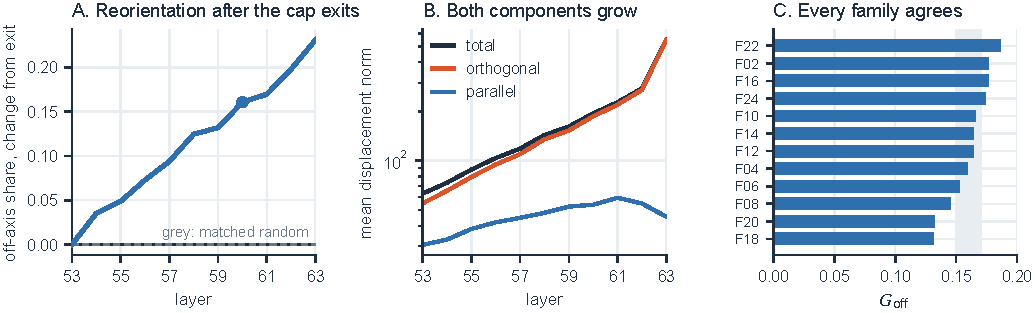
\includegraphics[width=\textwidth]{figures/supplement-propagation.pdf}
\caption{Downstream propagation on uncapped-source traces. (A) Change in off-axis energy share relative to the layer-53 cap exit, for p25 (solid) and for the four schedule-, token-, and norm-matched random-direction references (grey dashed); the marked point at layer 60 is $G_{\mathrm{off}}$. The references stay flat. (B) Mean absolute displacement norms from the cap exit on a logarithmic scale: total, the component orthogonal to the exit direction, and the component parallel to it. (C) Per-family $G_{\mathrm{off}}$, sorted; the shaded band is the pooled 95\% family-cluster interval. All 12 families are positive, from $0.131$ to $0.187$.}
\label{fig:supp-propagation}
\end{figure*}

Arm-level $G_{\mathrm{off}}$ estimates are $N=0.145$ $[0.132,0.160]$, $R=0.142$ $[0.127,0.157]$, $V=0.184$ $[0.174,0.194]$, and $F=0.172$ $[0.162,0.183]$. Reorientation is thus present with the target hidden and somewhat larger when an argument is present, matching the exposure pattern of Section~\ref{supp:contraction} rather than warrant validity: the $V$ and $F$ intervals overlap while both exceed $N$ and $R$.

\paragraph{Matched random-direction controls.}
The four references share the cap's firing schedule, token positions, and correction norm, and differ only in direction. Within the same RG1 stack they reproduce neither the propagation nor the behavioral effect (Table~\ref{tab:supp-randomctrl}, Figure~\ref{fig:supp-controls}B).

\begin{table*}[t]
\centering
\small
\begin{tabular}{lrlrl}
\toprule
Condition & $\Delta m_{\mathrm{general}}$ & 95\% CI & p25 $-$ reference & 95\% CI \\
\midrule
Released p25 & $+1.339$ & $[0.911,1.754]$ & \multicolumn{1}{c}{--} & \multicolumn{1}{c}{--} \\
Random seed-727 positive & $+0.595$ & $[0.323,0.863]$ & $+0.743$ & $[0.462,1.018]$ \\
Random seed-727 negative & $-0.098$ & $[-0.316,0.155]$ & $+1.436$ & $[0.941,1.893]$ \\
Random seed-728 positive & $-0.107$ & $[-0.292,0.090]$ & $+1.445$ & $[0.980,1.879]$ \\
Random seed-728 negative & $+0.289$ & $[0.025,0.538]$ & $+1.049$ & $[0.779,1.328]$ \\
\bottomrule
\end{tabular}
\caption{Behavioral effects of the matched random-direction references inside the common RG1 stack. Two of the four references move the broad margin on their own, so a norm-matched perturbation on this schedule is not inert; every paired p25-minus-reference contrast nonetheless excludes zero, and none of the references reproduces the off-axis reorientation. The comparison is specific to these four directions, not to the space of all directions.}
\label{tab:supp-randomctrl}
\end{table*}

This is the control that makes the p25 curve interpretable, and it is also the control that bounds the claim: the released direction is not merely a generic perturbation of this size, but neither is an arbitrary direction of the same size behaviorally inert.

\paragraph{Auxiliary validity probe.}
The family-held-out linear probe at layer 60 decodes $V/F$ validity in both conditions: ROC--AUC $0.769$ uncapped and $0.767$ under p25, balanced accuracy $0.688$ and $0.708$, against a text-only TF--IDF baseline at chance (AUC $0.511$, balanced accuracy $0.500$). Significance is assessed by exhausting all $2^{12}=4096$ family-label sign flips, giving $p=0.0144$ uncapped, $p=0.0022$ under p25, and $p=0.938$ for the text baseline. Per-family balanced accuracies (Figure~\ref{fig:supp-controls}C) are heterogeneous---two families sit at chance in both conditions and three reach $1.0$---so the pooled figure is not carried by a uniform effect. The probe was not a preregistered causal endpoint. It establishes condition-wise linear decodability, not a shared code across conditions and not causal use by the answer policy.

\begin{figure*}[t]
\centering
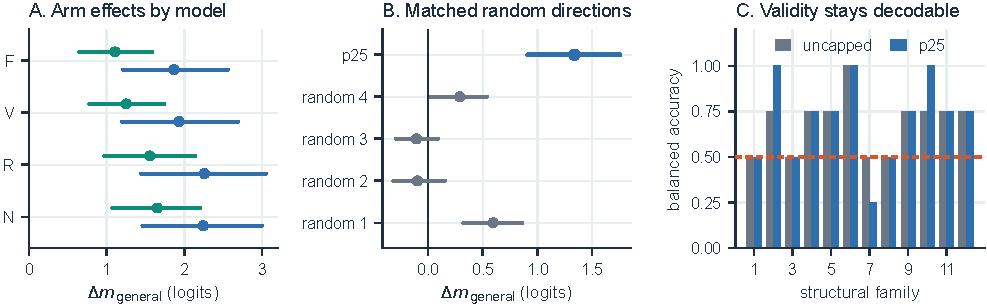
\includegraphics[width=\textwidth]{figures/supplement-controls.pdf}
\caption{Controls behind the mechanistic claims. (A) Arm-level broad-margin effects for the matched forced-choice audit, with 95\% family-cluster intervals; Qwen is blue and Llama is green, and every arm is positive in both configurations. (B) Broad-margin effects of the released cap and of the four schedule-, token-, and norm-matched random-direction references inside the RG1 stack. (C) Per-family balanced accuracy of the family-held-out $V/F$ probe at layer 60, uncapped in grey and under p25 in blue; the dashed line is chance.}
\label{fig:supp-controls}
\end{figure*}

\subsection{Affine contraction of the answer head}
\label{supp:contraction}

This analysis was added in response to a generic score-scaling alternative: if capping merely rescaled the option-logit vector, a positive $\Delta m_{\mathrm{general}}$ would follow from the initial answer's existing advantage without any redistribution among options.

\paragraph{Fit.}
For each paired item we take the four recorded option logits at the frozen answer position under the uncapped and p25 conditions and fit an ordinary least-squares line across options,
\begin{equation}
\ell^{\mathrm{p25}}_{o}=a\,\ell^{\mathrm{unc}}_{o}+b+\varepsilon_{o},\qquad o\in\{A,B,C,D\}.
\end{equation}
The initial answer $a_0$ is always the frozen \texttt{initial\_answer} recorded with the item, never the uncapped argmax; the two disagree on $14.6\%$--$32.6\%$ of items depending on assay, and using the argmax inflates the affine-explained share. Because every margin defined in the main paper is a contrast of logits, the intercept cancels exactly, leaving
\begin{equation}
\Delta m_{\mathrm{general}}=(a-1)\,m^{\mathrm{unc}}_{\mathrm{general}}+\varepsilon,
\end{equation}
where $\varepsilon$ collects the non-affine part. The \emph{affine-explained share} reported below is the ratio of the mean affine prediction to the mean observed $\Delta m_{\mathrm{general}}$ within a stratum; it is a descriptive decomposition, not a test.

\paragraph{Assay-level fits.}
Median $a$ and median $R^{2}$: RG1 fixed-trace replay (Qwen, $n=192$) $0.900$ / $0.9985$; matched forced-choice Qwen anchor ($n=96$) $0.442$ / $0.9412$; matched forced-choice Llama ($n=96$) $0.523$ / $0.9281$; new-salt generation (Qwen, $n=95$) $0.863$ / $0.9947$; CEDAR-Social $AO$ and $S$ ($n=600$ each) $0.910$ and $0.889$ / $0.997$. The fraction of items with $a<1$ ranges from $87.5\%$ to $98.2\%$.

\paragraph{Affine-explained share by arm.}
With the proposed target hidden, the affine term accounts for essentially all of the broad shift; wherever an argument is present, an arm-dependent non-affine component remains.

\begin{center}
\small
\begin{tabular}{@{}lrrrr@{}}
\toprule
Assay & $N$ & $R$ & $V$ & $F$ \\
\midrule
RG1 fixed trace & $102.5$ & $102.3$ & $217.9$ & $102.3$ \\
New salt & $100.4$ & $105.1$ & $-167.6$ & $157.2$ \\
Qwen forced choice & $100.0$ & $98.7$ & $64.4$ & $84.5$ \\
Llama forced choice & $99.9$ & $97.3$ & $63.8$ & $80.9$ \\
\bottomrule
\end{tabular}
\end{center}

\noindent Percentages of the observed mean $\Delta m_{\mathrm{general}}$. Values far from $100$ in the $V$ and $F$ columns indicate that the affine term is not a sufficient description once an argument is present; the $V$ entries for RG1 and new salt correspond to small observed means with opposite sign to the affine prediction and should be read as sign disagreement rather than as a magnitude.

\paragraph{Arm-level contraction and non-affine residual.}
Under the frozen trace, where the visible reasoning is token-identical across arms, contraction is nearly uniform: $N=0.902$, $R=0.901$, $V=0.908$, $F=0.896$. No equivalence test was prespecified, so this is an unresolved difference rather than demonstrated invariance. Under natural generation (new salt, 12-family cluster bootstrap, 20{,}000 draws) the arms separate by whether an argument is present:
\begin{center}
\small
\begin{tabular}{@{}lrl@{}}
\toprule
Quantity & Estimate & 95\% CI \\
\midrule
$a_{N}$ & $0.9002$ & $[0.8746,0.9269]$ \\
$a_{R}$ & $0.9157$ & $[0.8935,0.9369]$ \\
$a_{V}$ & $0.7032$ & $[0.5843,0.8060]$ \\
$a_{F}$ & $0.5889$ & $[0.4785,0.7047]$ \\
\midrule
$a_{V}-a_{R}$ & $-0.2124$ & $[-0.3416,-0.0984]$ \\
$a_{F}-a_{N}$ & $-0.3113$ & $[-0.4193,-0.2060]$ \\
$a_{V}-a_{F}$ & $+0.1144$ & $[-0.0983,+0.3095]$ \\
$\varepsilon_{V}-\varepsilon_{R}$ & $+1.4597$ & $[+0.7571,+2.3176]$ \\
$\varepsilon_{F}-\varepsilon_{R}$ & $+2.2561$ & $[+1.4344,+3.0635]$ \\
$\varepsilon_{V}-\varepsilon_{F}$ & $-0.7964$ & $[-2.1817,+0.7800]$ \\
\bottomrule
\end{tabular}
\end{center}
\noindent Mean $|\varepsilon|$ is ordered $V>F>R>N$ in both released configurations (Qwen $0.385/0.271/0.152/0.121$; Llama $0.315/0.254/0.162/0.134$) and $V>F>N>R$ under the frozen trace ($V$ $0.304$, $F$ $0.284$, $N$ $0.238$, $R$ $0.231$). These six contrasts are post-hoc and were not corrected for multiplicity; no LOFO or small-cluster sensitivity analysis accompanies them.

\paragraph{Exposure diagnostics.}
Cumulative above-threshold correction, per-position trigger rate, and triggerable position count by arm: $N$ $39{,}413$ / $0.5653$ / $7{,}041$; $R$ $40{,}101$ / $0.5561$ / $7{,}248$; $V$ $70{,}091$ / $0.5832$ / $12{,}122$; $F$ $66{,}841$ / $0.5856$ / $11{,}447$. Contrasts on cumulative correction: $F-R=+26{,}740$ $[+20{,}606,+33{,}018]$, $V-R=+29{,}990$ $[+24{,}547,+36{,}025]$, $V-F=+3{,}250$ $[-3{,}033,+9{,}706]$. Across items, cumulative correction and contraction correlate at $r=-0.463$ and position count and contraction at $r=-0.450$. The trigger rate is essentially constant across arms, so the exposure difference is driven by trajectory length rather than by a change in how often the operator fires. The available diagnostics resolve no $V$-versus-$F$ difference in exposure, contraction, or residual. Because no equivalence bound was prespecified, this means that unequal argument length was not observed to differ between the two argument arms, not that it has been excluded as a contributor. This is an observational association; no length-matched target-hidden control and no formal mediation analysis were run, so the exposure account is compatibility evidence rather than an identified causal chain.

\paragraph{Controls.}
A no-op repetition of the same forward pass returns $a=1.0000$ ($a<1$ on $41.7\%$ of items, consistent with numerical noise), so the contraction is not an artifact of the measurement or caching path. Of four schedule-, token-, and norm-matched random directions, two contract ($0.934$, $0.953$) and two do not ($1.002$, $0.998$). Contraction is therefore not specific to the Assistant direction; p25 produces the largest one among the interventions tested here.

\paragraph{Boundaries.}
The fit uses the four recorded option logits per item, so within-item $R^{2}$ is optimistic and a full-vocabulary refit is the natural extension. The CEDAR-Social primary estimands are target-minus-initial and $S-AO$, for which the affine term accounts for roughly $57\%$ ($AO$) and $26\%$ ($S$) and a non-affine remainder of about $-0.19$ persists in $S-AO$; the Social result is therefore not reduced to contraction. A first principal component of the centred logit difference explains $37$--$51\%$ of its variance against $44$--$54\%$ for matched random references, so there is no evidence for a single shared readout direction. This subsection describes the answer head under the tested regimes; it does not establish that a bounded, layer-local edit must act as a global change of readout scale, and that step remains part of the conjecture in the main paper.

\section{Development History and Hypothesis Revisions}
\label{supp:history}

The final assays were not selected after a single successful pilot.  Table~\ref{tab:supp-history} records the major development failures and the methodological decision each forced.  These stages are included to make the research path auditable. No row in the table is confirmatory: the development bank is exploratory, the new-salt bank is a same-family re-instantiation with one missing continuous pair, and the claim status of every estimate used in the paper is given in Section~\ref{supp:reproducibility}.

\begin{table*}[t]
\centering
\small
\begin{tabularx}{\textwidth}{L{1.65cm}L{2.1cm}L{3.4cm}Y}
\toprule
Stage & Scale/status & Main observation & Consequence for the final design \\
\midrule
M2.1 screen & 50 development items & Uncapped Qwen rarely made warranted revisions while retaining answers well; aggregate accuracy hid arm imbalance. & Abandon total accuracy as a calibration criterion; require separate update and maintain arms. \\
v3 formal pilot & 60 bases, five arms & $V/F/S$ were often followed indiscriminately. & Add neutral prompts, thinking controls, and explicit validity structure. \\
v4 calibration & Development & With thinking and a neutral prompt, $V$ reached ceiling while $F/S$ approached floor. & Stop treating surface complexity as behavioral difficulty. \\
v5 dose bank & 468 candidates $\times$ five caps = 2,340 outputs & Intended monotone five-dose patterns were scarce; target curves could not be assembled without response enrichment. & Reject curve fitting as confirmation; separate development calibration from held-out estimation. \\
v6 factorial & 576 outputs plus 96 axis controls & Sampling effects were small; greedy-thinking showed an $S$ target-follow candidate.  Axis positive controls passed in both thinking regimes. & Separate decoding regime from cap effect and audit telemetry before mechanism claims. \\
Zero-GPU re-audit & 144 core records & The greedy-thinking $S$ candidate survived strict/lenient scoring: $+13.89$ pp, family CI $[5.56,25.00]$. & Treat as a candidate, not ``sycophancy''; build held-out and cue ablation. \\
C1/V7 & 48 bases, 384 generations & $S$ target following $+18.75$ pp, $AO=0$; $V=-4.17$ pp. & Prompt cue became a plausible confound. \\
V7.1 cue ablation & 288 generations & No-cue $S$ effect $+6.25$ pp with CI spanning zero; six uncapped truncations. & Replace free generation as the primary Social readout with fixed short-answer logits. \\
C2/V8 & 600 direct pairs; 240 free pairs & Stable direct $S-AO=-0.786$ logits but zero free-generation SocialExcess. & Make margin--choice dissociation explicit and keep Social separate from Evidence. \\
Generator feasibility/hardening & 16-route comparison; 48 final bases & Solver certification, error balance, and deterministic rebuilding passed; naturalization required two revisions. & Freeze hybrid generator and human naturalization gate before Qwen. \\
Evidence development & 192 generations & $V$ and $F$ target following rose together; broad margin moved in all arms. & Replace ``benefit versus cost'' with reason-selectivity and general-displacement estimands. \\
New salt & 192 scheduled; 95/96 continuous pairs & Aggregate displacement repeated while categorical $V/F$ allocation changed. & Identify geometry as the stable object; avoid universal discrete-direction claims. \\
E0/E1 & Telemetry reanalysis and within-item sampling & Apparent late-decode resistance signature collapsed after length matching. & Reject the selective-resistance-state account. \\
E2B & 384 fixed-trace forwards & Positive displacement survived token-identical replay; no argmax changed. & Visible chain-of-thought alteration is not required for the continuous shift. \\
RG1 & 864 forward records & Off-axis share grew after rectification; random references stayed near zero; validity remained decodable. & Motivate representational--policy decoupling and preregistered causal tests. \\
\bottomrule
\end{tabularx}
\caption{Hypothesis and assay ledger. Counts are completed model outputs or forward passes.  ``Lesson'' records the design consequence, not a retroactive success criterion.}
\label{tab:supp-history}
\end{table*}

\subsection{Boundary analysis}

We also tested whether absolute uncapped margin universally predicts a paired choice flip.  A pooled clustered logistic analysis gave a negative slope of $-0.923$ ($[-1.457,-0.588]$), but the relation was driven by forced-choice PhilPapers.  Removing that dataset changed the slope to $+0.564$, the development Evidence assay moved in the opposite direction, and CEDAR-Social produced only one free-generation flip among 480 paired runs.  The boundary account therefore received Gate B: it is useful for interpreting forced-choice flips, but it is not a dataset-general explanation of all discrete effects.  The main paper accordingly states that discrete expression depends on surrounding decision geometry without claiming a universal absolute-margin law.

\subsection{Open items}

Table~\ref{tab:supp-open} lists the tests this account invites. Two analysis choices are worth stating explicitly because they bound what the contraction result means. The initial answer $a_0$ is always the frozen \texttt{initial\_answer} recorded with each item rather than the uncapped argmax; the two differ on a substantial fraction of items, and only the frozen field gives the estimand defined in the main paper. Separately, the capped-minus-uncapped logit difference is not dominated by one shared direction: its first principal component explains $37$--$51\%$ of the variance against $44$--$54\%$ for matched random references, so we describe the effect as an item-wise contraction of the answer head and not as a single global readout change.


\begin{table*}[t]
\centering
\small
\begin{tabularx}{\textwidth}{@{}L{4.6cm}L{2.4cm}Y@{}}
\toprule
Open item & Type & What it would change \\
\midrule
Unseen structural families and natural arguments & New experiment & Would move the recurrence claim from within-grammar validation to structural generalisation. \\
Cross-condition probe transfer and bidirectional patching & New experiment & Would decide representational--policy decoupling; the main paper states both as prospective tests. \\
Length-matched target-hidden control & New experiment & Would upgrade the exposure account from compatibility evidence to an identified mediator. \\
Full-vocabulary refit of the contraction & Re-recording & Would remove the four-point, two-parameter optimism in $R^{2}$. \\
Persona benefit measured in the tested stacks & New experiment & Would permit a benefit-matched controller comparison, which no claim here requires. \\
\bottomrule
\end{tabularx}
\caption{Open items. Each is a test the account invites rather than a gap it depends on: every claim in the main paper is scoped so that it does not turn on the outcome of any row here.}
\label{tab:supp-open}
\end{table*}

\section{Controller Implications of Representational--Policy Decoupling}
\label{supp:controller}

\subsection{Derivation of the observed signature under decoupling}

Representational--policy decoupling states that an intervention can preserve representational content while altering the revision policy that reads it. Each element of the reported signature follows. Target-hidden prompts move because what changed is the geometry of the current answer rather than attraction to a proposed one. The $V$ and $F$ arms need not separate because the change is graded by how much correction the operator applied rather than by warrant validity. Different banks yield different discrete revisions because one continuous displacement meets different local decision boundaries. And the effect leaves the coordinate on which it was imposed because the downstream remixing is what carries it. Validity information is not removed under this account; it is no longer read the same way, which is why condition-wise decodability at layer 60 coexists with a moved answer distribution.

Concretely, a probe fitted on uncapped layer-60 states should decode validity from p25 states and back if the code is preserved; failure in either direction would favour re-encoding or information loss over decoupling. Patching the corresponding route from uncapped into capped inference should restore part of the $V-F$ selectivity without freezing revision in general; no recovery would place the change upstream of the route we identify.

\subsection{Axis-conditioned gain redistribution: full statement and predictions}

The conjecture generalizes the account beyond a percentile cap to any intervention acting on a single direction in activation space. It holds that such an intervention does not add or remove a concept, but reweights the relative decision gain of many downstream pathways at once, graded by how strongly each pathway is coupled to the intervened axis: pathways bound to that axis gain share of the final decision, while weakly coupled pathways keep their content and lose influence over it. Because the operator fires repeatedly and its total correction grows with the length of what the model produces, this instantaneous reweighting accumulates into a persistent policy bias, which is why an inference-time edit can behave like a low-rank parameter change rather than a local nudge. The exposure-graded contraction reported above is the shape this predicts at an answer head, and a scalar rescaling is only its simplest realization.

For an Assistant direction, the pathways that gain are plausibly identity maintenance, policy compliance, and resistance to role shift; the pathway that loses is whether a particular inference step is sound. Prior work establishes the separate components: stronger activation control has been linked to reduced general utility \citep{xu2026steering}, steering to attention rerouting away from evidence tokens \citep{luo2026focus}, a single residual direction to whether reasoning or memorization governs an answer \citep{hong2025reasoning}, and feature interventions to diffuse rather than reusable single-direction effects \citep{hoang2026sae}. Their conjunction, not any one of them, is what is new here. Norm- and dose-matched interventions along axes other than the Assistant direction, cross-condition probes, and activation patching are its direct tests; a uniform rather than coupling-graded loss of influence would break it.

The hypothesis in the main paper motivates a controller that separates drift detection from the actuation applied after a trigger.  This extends the general goal of reducing activation-steering side effects and conditioning intervention strength on context \citep{stickland2024steering,lee2025programming} to a different constraint: preserving evidence-sensitive revision.  Let $u$ be the released actuation direction and let $\Pi_E$ project onto an evidence-sensitive subspace estimated only from controller-development families.  A protected direction is
\begin{equation}
u_{\perp}=\frac{(I-\Pi_E)u}{\lVert(I-\Pi_E)u\rVert_2}.
\end{equation}
This construction does not assume that a single linear subspace captures all valid reasoning.  It states a testable design principle: a persona controller should avoid removing components shown to support warranted revision.

A concrete comparison ladder separates three choices.  L0 is the released one-sided threshold cap.  L1 retains the released trigger but redirects the corrective update onto $u_{\perp}$, separating detection from actuation.  L2 uses the protected decomposition for both gating and actuation, so evidence-sensitive movement alone cannot satisfy the removal rule.  Subspace estimation, thresholds, layers, and matching tolerances must be selected only on controller-development families and frozen before held-out evaluation.

The operating point must be benefit-matched.  A variant first has to retain the same independently measured persona benefit, or the same CEDAR-Social attenuation when persona evaluation is unavailable.  Within that constraint, valid updating should be preserved, fallacious updating should not increase, target-hidden broad movement should shrink, and output integrity, exposure, capability, and compute should remain acceptable.  This ladder is a design consequence of the present hypothesis, not an evaluated result.

Cross-condition probe transfer and bidirectional activation patching provide the immediate mechanism tests.  Transfer asks whether capped and uncapped inference share a usable validity code; patching asks whether that code causally participates in revision.   The patching design must freeze its corruption, metric, layer blocks, and controls because these choices can materially alter localization conclusions \citep{zhang2023patching}.  New structural families, natural argument datasets, and additional released model--axis pairs test transport beyond the present grammar and configurations.

\section{Artifact Inventory and Reproduction Contract}
\label{supp:reproducibility}

\begin{table*}[t]
\centering
\small
\renewcommand{\arraystretch}{1.12}
\begin{tabularx}{\textwidth}{@{}L{3.2cm}YY@{}}
\toprule
Archive block & Contents & Principal validation \\
\midrule
\path{data/evidence_development_bank} & Measurement bases, construction audit, family allocation, balance and rebuild reports, tokenizer preflight & 48/48 bases; 288/288 arms; deterministic rebuild \\
\path{data/evidence_certified_pool} & Certified candidate worlds, proof traces, countermodels, solver outputs & Dual-solver agreement; unique gold; single certified fault \\
\path{data/evidence_validation_inputs} & Frozen prompts, option maps, and gates for the development assay & Target concealment in $N/R$; bijective option maps \\
\path{data/phase_validity_inputs} & Frozen prompts and gates for the phase and validity assays & Same base set; separate response contracts \\
\path{data/evidence_new_salt} & Regenerated bases and arms, construction audits, review, proofs, and countermodels & Same frozen family grammar; new names, option maps, and salt \\
\path{data/social_inputs} & Licensed source snapshot, paired $AO/S$ inputs, construction audits, and review record & Source validation; pairing and prohibited-cue gates; single-review limitation retained \\
\path{runs/evidence_development} & Per-item records, option logits, finish reasons, parse status, analysis JSON & Formal audit; missing-output ledger; option-space integrity \\
\path{runs/evidence_new_salt} & Same-family re-instantiation records and analysis JSON & 95/96 complete continuous pairs; tipping sensitivity \\
\path{runs/phase_and_validity} & Prefill-only, decode-only, full-cap, and validity-assay records & Phase contrasts; independent validity readout \\
\path{runs/fixed_trace_replay} & Frozen token-sequence hashes and lengths, cache-faithful replay records, replay option logits, and fidelity report & 192/192 replay fidelity; no hook leaks or nonfinite values \\
\path{runs/social} & Direct and free-generation records and analysis JSON & Pair and target equality; transition and completion audits \\
\path{runs/calibration_steering}, \path{runs/calibration_cap} & Signed-dose steering and cap-exposure records with token diagnostics & Dose curve; exposure; vocabulary-wide integrity \\
\path{runs/downstream_propagation} & Layerwise displacement components per record, propagation summary, probe scores & 864/864 forwards; family-held-out probe; matched random references \\
\path{runs/cross_model} & Matched forced-choice records and pooled/arm estimates for both configurations & Shared prompts and scoring contract; model-native scales; portable CPU recomputation \\
\path{runs/scale_contraction} & Machine-readable affine fits, arm contrasts, exposure diagnostics, and controls & Frozen initial answer; recorded logits only; no model rerun \\
\path{code} & Data builders, validators, runners, analyzers, environment files, and figure scripts & Syntax audit; portable CPU recomputation for transport and contraction \\
\bottomrule
\end{tabularx}
\caption{Anonymous artifact inventory. The release package maps these stable blocks to files after review. Raw model weights and intervention vectors are not redistributed; the licensed SycoBench source snapshot and its license are included.}
\label{tab:supp-artifacts}
\end{table*}

\subsection{Checklist-facing reproducibility details}

Table~\ref{tab:supp-artifacts} lists the archive blocks and their principal validations. The release package includes: (i) machine-readable train-free data-generation and validation code; (ii) all prompts and response contracts; (iii) the public model and tokenizer identifiers used; (iv) the identifiers of the released axis and threshold assets, which remain distributed by their original authors; (v) solver versions and proof/countermodel traces; (vi) software and hardware manifests; (vii) smoke and formal run commands; (viii) row-level results, finish reasons, parse status, and logits; (ix) bootstrap seeds and complete estimate ledgers; and (x) deterministic delivery manifests.  No training, parameter optimization, or checkpoint selection is performed.  Hyperparameters that could affect inference---thinking toggle, greedy/forced-choice regime, seed, batch size, maximum generation length, precision, attention implementation, layer window, threshold, and token phase---are bound to each result block. The root delivery manifest is computed after anonymization; a separate sanitization ledger binds source hashes to delivered hashes, so pre-anonymization scientific manifests are not misused as archive-integrity checks.

The Evidence data, generator, and evaluation code are novel artifacts and will be released upon publication. SycoBench-derived records retain source identifiers and license metadata, and the anonymous archive includes the frozen source snapshot under its CC-BY-4.0 license together with the deterministic paired-prompt builder. The submission contains no author names, affiliations, identifying links, private paths, hardware UUIDs, or project version-control history.

\subsection{Claim-status boundaries}

The development Evidence assay is exploratory.  The new-salt result is a new instance sample from the same families, with one missing continuous pair.  CEDAR-Social has deterministic pairing audits but only one human reviewer.  Fixed-trace replay is a conditional continuous assay and produces no discrete answer changes.  RG1 shows downstream off-axis propagation relative to matched references; the auxiliary probe shows decodability, not causal use.  The affine-contraction decomposition of the answer head is a descriptive reanalysis of recorded option logits, not a preregistered endpoint, and its arm-level contrasts are post-hoc; axis-conditioned gain redistribution is stated as a conjecture and is not tested. The matched Llama result transports the broad displacement to a second released model--axis configuration under a common forced-choice regime, but does not isolate model identity from configuration.  These boundaries are encoded in the claim register and preserved in the manuscript wording.

\bibliography{references}

\end{document}
